\section{ DQN 算法}

我们知道求解强化学习的一种思路就是优化状态价值函数 $V(s)$ 或动作价值函数 $Q(s,a)$,而传统强化学习算法是以表格的形式存储这些价值函数的,这导致最终优化的对象本身就具有一定的局限性。首先表格形式的价值函数是离散的,存储的状态之间比较独立,对于一些近似状态的拟合就难以体现出关联性。以学生上下课为例,对于学生这个智能体来讲,数学课和物理课这两种状态其实应该是近似的,因为对于考高分这个长期目标来说,数学课和物理课具有类似的价值(都涉及复杂的公式和逻辑),换句话说对应的状态-价值函数应当类似。但是如果用表格形式存储的话,在更新价值函数的过程中是体现不出来这些关联性的。其次表格能够存储的状态-动作对是有限的,这受限于计算机的内存空间,这样一来在实际的强化学习任务中往往涉及成千上万个状态-动作对,如果都用表格来存储的话,会增加很多的计算和内存成本。在这种情况下,最好的办法就是换一种价值函数的表示形式,而深度神经网络就能很好地解决这个问题。深度神经网络本质上就是一个复杂的非线性函数,比较契合价值函数本身的定义,此外使用深度神经网络也能顺便解析一些复杂的状态及其内在的关联性,例如解决图像输入的卷积神经网络等等,因此目前主流的强化学习算法都是以深度神经网络为基础的算法,我们称作深度强化学习算法(DRL,Deep Reinforcement Learning)。

\subsection{深度学习基础}

在本章中会详细讲解一种经典的 DRL 算法,即 DQN 算法,在介绍该算法之前我们先简单了解一些深度学习的基础。注意,这里只是简单做一个入门的铺垫,如果读者们后面想深入做强化学习算法研究或者相关应用时,还是有必要进一步了解更多的深度网络模型的,例如能够识别图像状态输入的卷积神经网络、解析时间序列状态输入的循环神经网络等等。
\subsubsection{线性模型}

首先介绍线性模型,线性模型是最简单的一类机器学习模型,可以将其视为单层的神经网络。在线性模型中最基础的两个模型就是线性回归和逻辑回归,通常分别用于解决回归和分类问题,尽管后者也可以用来解决回归问题。回归模型的输出是一个连续的值,而分类模型的输出是离散的值,用于表示分类。本质上来说回归模型和分类模型是一样的,分类模型可以将回归模型离散化,例如本节将要讲的逻辑回归就是在线性回归的基础上增加了一个 sigmoid 函数对其进行了离散化。顺便提一句,回归模型也可以将分类模型连续化,通常见于贝叶斯模型中,但这在强化学习中并不常用。

{\bfseries 线性回归。} 以Kaggle入门竞赛项目房价预测为例,一套房子有$m$个特征,例如建造年份、房子面积等等,把这$m$个特征用向量表示,如下:

\begin{equation}
    % \label{eq:softmax_act}$
    \boldsymbol{x}=\left[x_1, x_2, \cdots, x_m\right]
\end{equation}

我们可以用线性模型来拟合这$m$个特征和房价的关系,如下:

\begin{equation}
    % \label{eq:softmax_act}$
    f(\boldsymbol{x} ; \boldsymbol{w}, b) = w_1 x_1+w_2 x_2+\cdots+w_m x_m+b = \boldsymbol{w}^T \boldsymbol{x}+b
\end{equation}

其中$\boldsymbol{w}$和$b$是模型的参数,$f(\boldsymbol{x} ; \boldsymbol{w}, b)$是模型的输出,也就是我们要预测的房价。出于简化考虑,通常我们会用一个符号$\boldsymbol{\theta}$来表示$\boldsymbol{w}$和$b$,如下:

\begin{equation}
    % \label{eq:softmax_act}$
    f^{\theta}(\boldsymbol{x}) = \boldsymbol{\theta}^T \boldsymbol{x}
\end{equation}

我们的目的是求得一组最优的参数$\boldsymbol{\theta^{*}}$,使得该模型能够根据房屋的$m$个特征预测对应的房价。我们一般利用历史数据来近似求解最优参数,这个过程就叫做训练。注意这里是近似求解,因为几乎所有机器学习模型都无法找到一种方法能够获得绝对的最优解,甚至也不一定存在绝对最优解,有些方法甚至很容易陷入局部最小值的问题中。训练的方法,或者说求解模型参数的方法理论上来说有很多种,比如这里线性模型可以用最小二乘法来求解,另外有些模型可以用牛顿法来求解,而目前普遍流行的优化方法就是梯度下降。梯度下降方法泛化能力很强,能够基于梯度下降求解很多种模型,该方法的本质是一阶泰勒展开,顺便提一句,牛顿法则是二阶泰勒展开。

{\bfseries 逻辑回归。} 对于分类问题,其预测目标不再是连续的值,而可能是二元变量,要么等于0,要么等于1,即最简单的二分类问题。这种情况下,我们可以用逻辑回归来解决,注意虽然逻辑回归名字里带有回归,但通常用于解决二分类问题而非回归问题。逻辑回归的思路也比较简单,如\figref{fig:logistic_struction}所示,就是在线性模型的后面增加一个sigmoid函数,我们一般称之为激活函数。逻辑回归模型其实可以看做神经网络模型的一个神经元,具体后面再展开说明。

\begin{figure}[hbt]
    \centering
    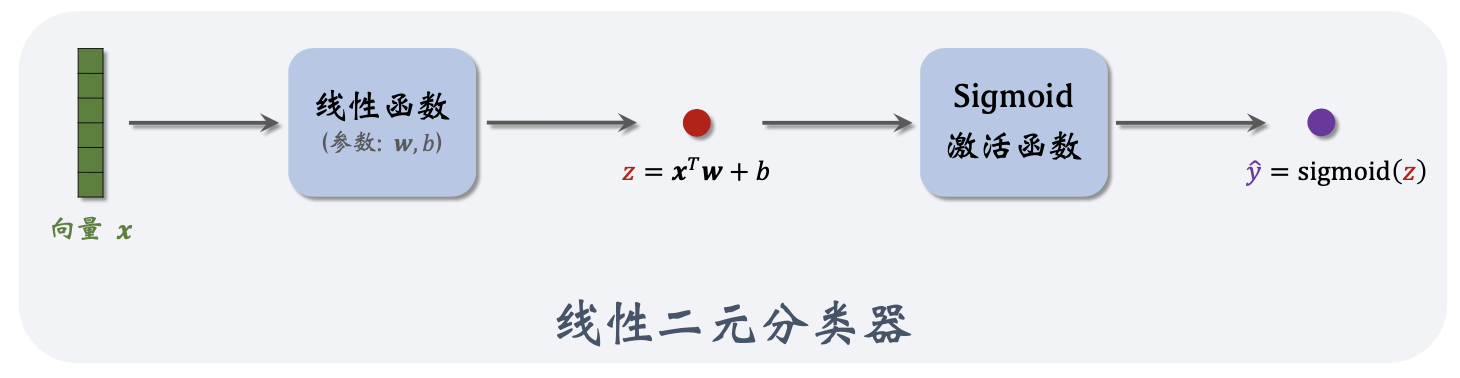
\includegraphics[width=0.5\linewidth]{ch4/figs/logistic_struction.png}
    \caption{逻辑回归,线性 Sigmoid 分类器的结构}
    \label{fig:logistic_struction}
\end{figure}

sigmoid 函数定义为:

\begin{equation}
    % \label{eq:softmax_act}$
    sigmoid(z) = \frac{1}{1+exp(-z)}
\end{equation}

如\figref{fig:sigmoid}所示,sigmoid 函数可以将输入的任意实数映射到$0-1$之间,对其输出的值进行判断,例如小于0.5我们认为预测的是类别0,反之是类别1,这样一来通过梯度下降来求解模型参数就可以用于实现二分类问题了。注意,虽然逻辑回归只是在线性回归模型基础上增加了一个激活函数,但两个模型是完全不同的,包括损失函数等等。线性回归的损失函数是均方差损失,而逻辑回归模型一般是交叉熵损失,这两种损失函数在深度学习和深度强化学习中都很常见,具体推导细节读者可自行翻阅相关资料。

\begin{figure}[hbt]
    \centering
    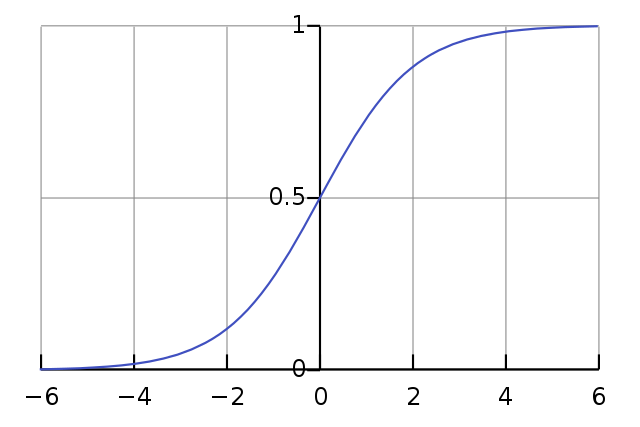
\includegraphics[width=0.5\linewidth]{ch4/figs/sigmoid.png}
    \caption{Sigmoid函数图像}
    \label{fig:sigmoid}
\end{figure}

\subsubsection{神经网络}

{\bfseries 全连接网络。} 全连接网络又称作多层感知机(multi-layer perceptron,MLP),是最基础的神经网络模型。它是基于生物神经网络的启发,将“线性函数+激活函数”这样的结构一层层堆叠(stack)组合成一个多层的网络模型,用于解决更复杂的问题。如\figref{fig:ann_vs_dnn}所示,线性函数可以看做生物神经网络的神经元,而激活函数就是神经元之间的突触结构。顺便说一句,生物神经网络是神奇且复杂的,人们也一直在尝试研究新的人工神经网络模型去模拟生物神经网络,例如脉冲神经网络,尽管目前这些模型还没有得到广泛地验证。

\begin{figure}[hbt]
    \centering
    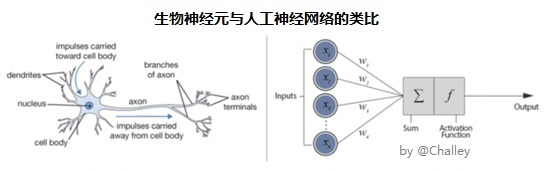
\includegraphics[width=0.5\linewidth]{ch4/figs/ann_vs_dnn.png}
    \caption{生物神经网络与人工神经网络的对比}
    \label{fig:ann_vs_dnn}
\end{figure}

记神经网络模型中上一层的输入向量为$\boldsymbol{x^{l-1}}\in \mathbb{R}^{d^{l-1}}$,其中第一层的输入也就是整个模型的输入可记为$\boldsymbol{x^0}$,每一个全连接层将上一层的输入映射到$\boldsymbol{x^{l}}\in \mathbb{R}^{d^{l}}$,也就是下一层的输入,具体定义为:

\begin{equation}
    \boldsymbol{x}^{l}=\sigma(\boldsymbol{z}), \quad \boldsymbol{z}=\boldsymbol{W} \boldsymbol{x^{l-1}}+\boldsymbol{b} = \boldsymbol{\theta} \boldsymbol{x^{l-1}}
\end{equation}

其中$\boldsymbol{W}\in \mathbb{R}^{d^{l-1} \times d^{l}}$是权重矩阵,$\boldsymbol{b}$为偏置矩阵,与线性模型类型,这两个参数我们通常看作一个参数$\boldsymbol{\theta}$。$\sigma(\cdot)$是激活函数,除了 Sigmoid 函数之外,还包括 Softmax 函数、ReLU 函数和 tanh 函数等等激活函数。其中最常用的是 ReLU 函数 和 tanh 函数,前者将神经元也就是线性函数的输出映射到$0-1$之间,后者则映射到$-1$到$1$之间。前面讲到,在强化学习中我们用神经网络来近似动作价值函数,动作价值函数的输入是状态,输出是各个动作对应的价值,在有些连续动作问题中比如汽车方向盘转动角度是$-90$度到$90$度之间,这种情况下使用 tanh 激活函数能够使得神经网络负值以便于更好地近似状态动作函数。顺便提一句,这里还有一种做法是我们可以把动作空间映射到正值的范围,例如$0$到$180$区间,这样一来对应的神经网络模型激活函数使用 ReLU 函数会更好些。

一个$l$层的神经网络模型可以表示为:
\begin{equation}
    \begin{split}
    第 1 层: \quad \boldsymbol{x}^{(1)}=\sigma_1\left(\boldsymbol{W}^{(1)} \boldsymbol{x}^{(0)}+\boldsymbol{b}^{(1)}\right),\\
    第 2 层: \quad \boldsymbol{x}^{(2)}=\sigma_2\left(\boldsymbol{W}^{(2)} \boldsymbol{x}^{(1)}+\boldsymbol{b}^{(2)}\right),\\
    \vdots \quad \vdots\\
    第 l 层: \quad \boldsymbol{x}^{(l)}=\sigma_l\left(\boldsymbol{W}^{(l)} \boldsymbol{x}^{(l-1)}+\boldsymbol{b}^{(l)}\right)\\
\end{split}
\end{equation}

求解神经网络模型参数的方法除了梯度下降之外,还涉及多层网络模型的正向传播和反向传播,具体细节在接下来的小节中展开。

{\bfseries 卷积神经网络。}

{\bfseries 循环神经网络。}


{\bfseries Transformer。}
\subsubsection{梯度下降}

TODO
\subsubsection{反向传播}
TODO
\subsection{ DQN 算法}

DQN 算法,英文全称 Deep Q-learning,顾名思义就是基于深度网络模型的 Q-learning 算法,主要由 DeepMind 公司于2013年和2015年分别提出的两篇论文来实现,即《Playing Atari with Deep Reinforcement Learning》和《Human-level Control through Deep Reinforcement Learning》。DQN 算法相对于 Q-learning 算法来说更新方法本质上是一样的,而 DQN 算法最重要的贡献之一就是本章节开头讲的,用神经网络替换表格的形式来近似动作价值函数$Q(\boldsymbol{s},\boldsymbol{a})$。

\begin{figure}[hbt]
    \centering
    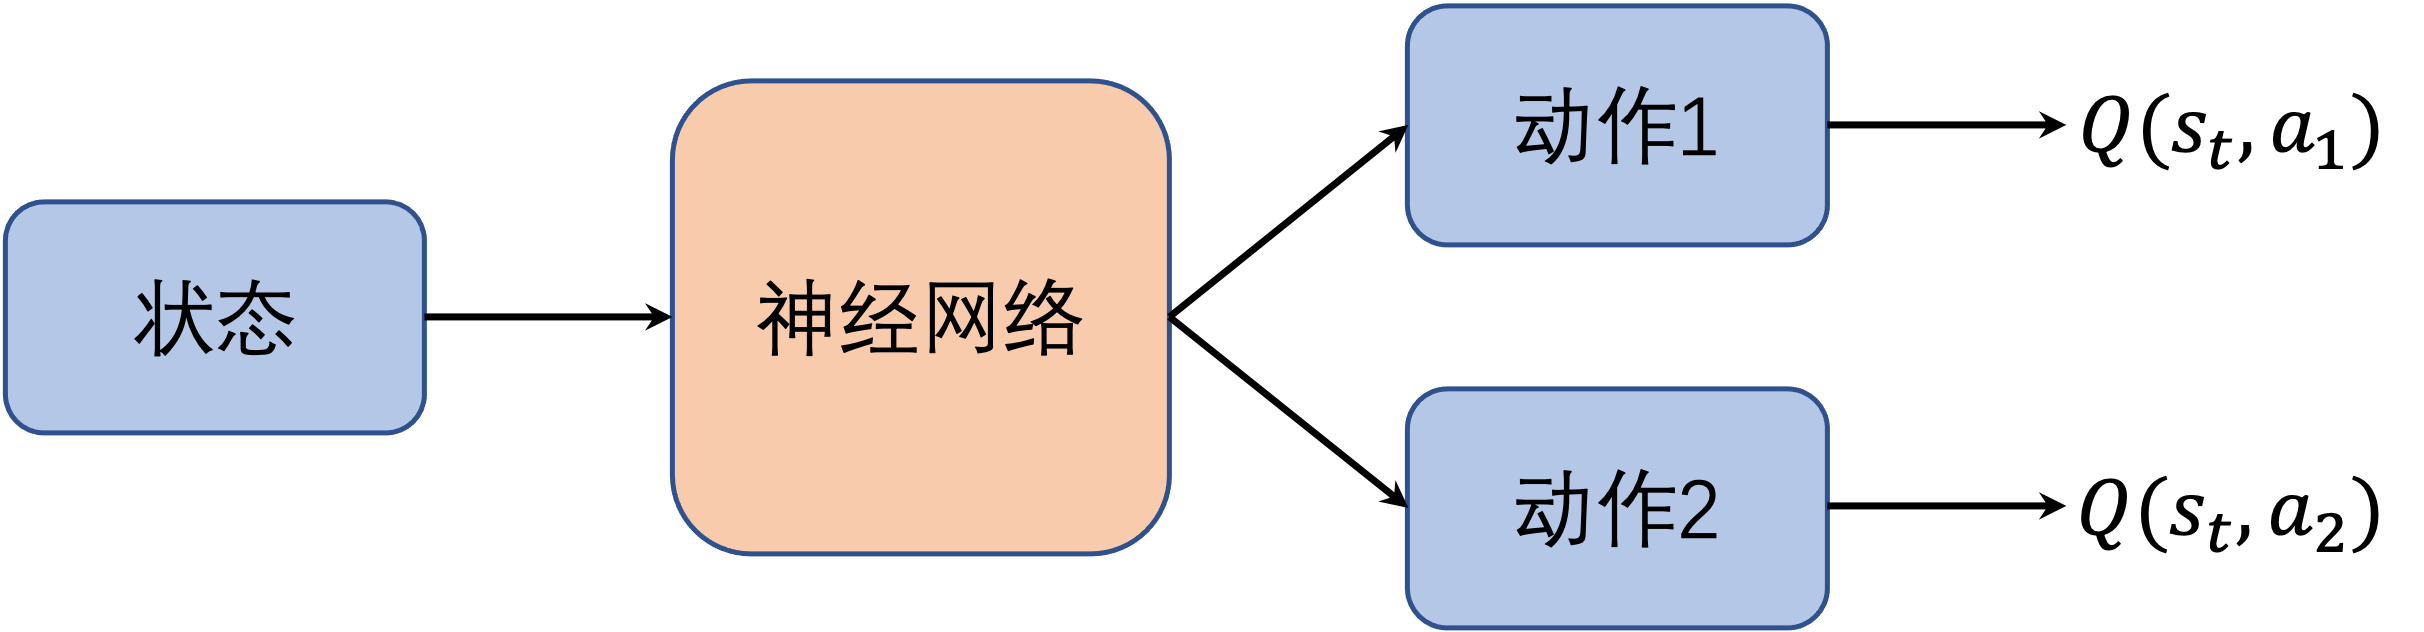
\includegraphics[width=0.5\linewidth]{ch4/figs/dqn_network.png}
    \caption{DQN 网络结构}
    \label{fig:dqn_network}
\end{figure}

如\figref{fig:dqn_network}所示,在 DQN 的网络模型中,我们将当前状态$s_t$作为输入,并输出动作空间中所有动作(假设这里只有两个动作,即1和2)对应的动作价值即$Q$值,我们记做$Q(s_t,\boldsymbol{a})$。对于其他状态,该网络模型同样可以输出所有动作对应的价值,这样一来神经网络近似的动作价值函数可以表示为$Q^{\theta}(\boldsymbol{s},\boldsymbol{a})$。其中$\theta$就是神经网络模型的参数,可以结合梯度下降的方法求解。

具体该怎么结合梯度下降来更新$Q$值呢?我们首先回顾一下 Q-learning 算法的更新公式如下:

\begin{equation}
    Q(s_t,a_t) \leftarrow Q(s_t,a_t)+\alpha[r_t+\gamma\max _{a}Q(s_{t+1},a)-Q(s_t,a_t)]
\end{equation}

我们注意到公式右边两项$r_t+\gamma\max _{a}Q(s_{t+1},a)$和$Q(s_t,a_t)$分别表示期望的$Q$值和实际的$Q$值,其中预测的$Q$值是用下一个状态对应$Q$值的最大值来近似的。换句话说,在更新$Q$值并达到收敛的过程中,期望的$Q$值也应该接近实际的$Q$值,即我们希望最小化$r_t+\gamma\max _{a}Q(s_{t+1},a)$和$Q(s_t,a_t)$之间的损失,其中$\alpha$是学习率,尽管优化参数的公式跟深度学习中梯度下降法优化参数的公式有一些区别(比如增加了$\gamma$和$r_t$等参数)。从这个角度上来看,强化学习跟深度学习的训练方式其实是一样的,不同的地方在于强化学习用于训练的样本(包括状态、动作和奖励等等)是与环境实时交互得到的,而深度学习则是事先准备好的训练集。当然训练方式类似并不代表强化学习和深度学习之间的区别就很小,本质上来说强化学习和深度学习解决的问题是完全不同的,前者用于解决序列决策问题,后者用于解决静态问题例如回归、分类、识别等等。在 Q-learning 中,我们是直接优化 Q 值的,而在 DQN 中使用神经网络来近似 Q 值,我们则需要优化网络模型对应的参数$\theta$,如下

\begin{equation}
    \begin{split}
    y_{i}= \begin{cases}r_{i} & \text {对于终止状态} s_{i} \\ r_{i}+\gamma \max _{a^{\prime}} Q\left(s_{i+1}, a^{\prime} ; \theta\right) & \text {对于非终止状态} s_{i}\end{cases}\\
    L(\theta)=\left(y_{i}-Q\left(s_{i}, a_{i} ; \theta\right)\right)^{2}\\
    \theta_i \leftarrow \theta_i - \alpha \nabla_{\theta_{i}} L_{i}\left(\theta_{i}\right)\\
\end{split}
\end{equation}

其中期望的Q值$y_{i}$增加了对终止状态和非终止状态的判断,这是因为当$s_t$为终止状态时,$Q(s_{t+1},a)$是不存在的($s_{t+1}$不存在),所以需要将其置0,在 Q-learning 中其实也需要有同样的操作,只是出于简化考虑没有列出。

\subsubsection{经验回放}

前面讲到,强化学习的训练方式是与环境实时交互得到样本然后进行训练的,在 Q-learning 中我们是每次交互一个样本,通常包含当前状态($state$)、当前动作($action$)、下一个状态($next\_state$)、是否为终止状态($done$),这样一个样本我们一般称之为一个状态转移(transition)。这种每次只交互一个样本并更新的方式会产生两个问题,首先是在强化学习问题中样本之间的关联性过强(从当前状态到下一个状态的过渡不可能是突变的,比如我们在吃饭时中间忽然加快速度张开血盆大口猛吃也不会导致我们的肚子一下子就鼓鼓的,会有一个相对缓慢的变化过程),会导致更新的过程不够稳定并且容易陷入局部最优解。本质上来说这其实就是随机梯度下降相对于单纯梯度下降的好处,只是在强化学习中体现得更为明显,因为强化学习前后两个样本的关联性往往比监督学习更紧密,从而导致训练的不稳定。另外一个问题是我们每次只看一个样本来更新,这在 DQN 算法中的劣势会更加明显,因为 DQN 算法是基于深度神经网络模型的。在深度学习的梯度下降中,我们知道如果在训练时每次遍历整个数据集并更新一次损失函数和梯度是会保证不错的收敛性的,但是计算开销会很大,这就是前面所说的批梯度下降方法(batch gradient descent)。但如果每次只看一个样本并更新梯度,尽管速度会提上去,但是会导致收敛性能不好,容易在最优点附近徘徊,于是有了一个折中的方法,即小批量梯度下降(mini-batch gradient descent)。鉴于这两个问题, DeepMind 公司 在论文中提出了一个经验回放的概念(replay buffer),这个经验回放的功能主要包括三个方面。首先是能够缓存一定量的状态转移即样本,此时 DQN 算法并不急着更新并累积一定的初始样本,就好比我们学习做饭炒菜一样,先把颠勺、抡刀、切菜、放调料等等都先零碎地试一遍。然后是每次更新的时候随机从经验回放中取出一个小批量的样本并更新策略,注意这里的随机和小批量以便保证我们存储动作价值函数的网络模型是小批量随机梯度下降的。最后要保证经验回放是具有一定的容量限制的,太小了会导致收集到的样本具有一定的局限性,太大了会失去经验本身的意义。这就好比我们在做自我规划一样,往往会根据自身经验制定一个三年或者五年计划,如果制定的计划周期太长比如制定一个二十年计划是没有任何意义的,因为二十年间的变数太多会导致制定的计划失去效用。类似的经验回放太大容易导致智能体在更新策略时可能会使用一些比较久远的样本,根据马尔可夫过程的性质,太过久远的样本对于当前状态的参考意义不大,就好比我们制定一个二十年当上小学校长的计划,等到十年过去后发现我们中间有太多的变数而身不由己,这样一来当初制定的二十年计划大概率就流产了。而小批量的样本更新就好比在三五年计划的基础上我们制定一个每周计划,每周行动并反思然后结合三五年计划或目标调整下一周的行动,这种方式往往是最高效的。到这里,我们又不得不感叹一句,生活中处处是强化学习!
\subsubsection{目标网络}

在 DQN 算法中还有一个重要的技巧,就是使用了一个每隔若干步才更新的目标网络,与之相对的,会有一个每步更新的网络,即每次从经验回放中采样到样本就更新网络参数,在本书中一般称之为策略网络。策略网络和目标网络结构都是相同的,都用于近似 Q 值,在实践中每隔若干步才把每步更新的策略网络参数复制给目标网络,这样做的好处是保证训练的稳定,避免 Q值 的估计发散。举一个典型的例子,这里的目标网络好比明朝的皇帝,而策略网络相当于皇帝手下的太监,每次皇帝在做一些行政决策时往往不急着下定论,会让太监们去收集一圈情报,然后集思广益再做决策。这样做的好处是显而易见的,比如皇帝要处决一个可能受冤的犯人时,如果一个太监收集到一个情报说这个犯人就是真凶的时候,如果皇帝是一个急性子可能就当初处决了,但如果这时候另外一个太监收集了一个更有力的证据证明刚才那个太监收集到的情报不可靠并能够证明该犯人无罪时,那么此时皇帝就已经犯下了一个无法挽回的过错。换句话说,如果当前有个小批量样本导致模型对 Q 值进行了较差的过估计,如果接下来从经验回放中提取到的样本正好连续几个都这样的,很有可能导致 Q 值的发散(它的青春小鸟一去不回来了)。再打个比方,我们玩 RPG 或者闯关类游戏,有些人为了破纪录经常存档(Save)和回档(Load),简称“SL”大法。只要我出了错,我不满意我就加载之前的存档,假设不允许加载呢,就像 DQN 算法一样训练过程中会退不了,这时候是不是搞两个档,一个档每帧都存一下,另外一个档打了不错的结果再存,也就是若干个间隔再存一下,到最后用间隔若干步数再存的档一般都比每帧都存的档好些呢。当然我们也可以再搞更多个档,也就是DQN增加多个目标网络,但是对于 DQN 算法来说没有多大必要,因为多几个网络效果不见得会好很多。


\subsubsection{探索策略}
\subsection{实战:DQN算法}


\subsection{关键词}
\subsection{习题}
\subsection{面试题}
\subsection{本章小结}